%--------------------
% Packages
% -------------------
\documentclass[11pt,english]{article}
\usepackage{amsfonts}
\usepackage[left=2.5cm,top=2cm,right=2.5cm,bottom=3cm,bindingoffset=0cm]{geometry}
\usepackage{amsmath, amsthm, amssymb}
\usepackage{tikz}
\usetikzlibrary{calc}
\usetikzlibrary{decorations.pathreplacing,calligraphy}
\usepackage{fancyhdr}
%\usepackage{currfile}
\usepackage{nicefrac}
\usepackage{cite}
\usepackage{graphicx}
\usepackage{caption}
\usepackage{longtable}
\usepackage{rotating}
\usepackage{lscape}
\usepackage{booktabs}
\usepackage{float}
\usepackage{placeins}
\usepackage{setspace}
\usepackage[font=itshape]{quoting}
\onehalfspacing
\usepackage{mathrsfs}
\usepackage{tcolorbox}
\usepackage{xcolor}
\usepackage{subcaption}
\usepackage{float}
\usepackage[multiple]{footmisc}
\usepackage[T1]{fontenc}
\usepackage[sc]{mathpazo}
\usepackage{listings}
\usepackage{longtable}
\definecolor{cmured}{RGB}{175,30,45}
\definecolor{macroblue}{RGB}{56,108,176}
\usepackage[format=plain,
            labelfont=bf,
            textfont=]{caption}
\usepackage[colorlinks=true,citecolor=macroblue,linkcolor=macroblue,urlcolor=macroblue]{hyperref}
\usepackage{varioref}
\usepackage{chngcntr}
\usepackage{datetime}

\definecolor{darkgreen}{RGB}{30,175,88}
\definecolor{darkblue}{RGB}{30,118,175}
\definecolor{maroon}{rgb}{0.66,0,0}
\definecolor{darkgreen}{rgb}{0,0.69,0}

%Counters
\newtheorem{theorem}{Theorem}[section] 
\newtheorem{proposition}{Proposition}
\newtheorem{lemma}{Lemma}
\newtheorem{corollary}{Corollary}
\newtheorem{assumption}{Assumption}
\newtheorem{axiom}{Axiom}
\newtheorem{case}{Case}
\newtheorem{claim}{Claim}
\newtheorem{condition}{Condition}
\newtheorem{definition}{Definition}
\newtheorem{example}{Example}
\newtheorem{notation}{Notation}
\newtheorem{remark}{Remark}


\hypersetup{ 	
pdfsubject = {},
pdftitle = {TidyTuesday Week 50},
pdfauthor = {Pranay Gundam},
linkcolor= macroblue
}


\title{\textbf{TidyTuesday Week 50}}
\author{Pranay Gundam}


%-----------------------
% Begin document
%-----------------------
\begin{document}

\maketitle

\tableofcontents

\section{Weekly Summary}


\section{Date: 2024-12-12}
\noindent \textbf{Series ID: WPU301601075} 

\noindent This series is titled Producer Price Index by Commodity: Transportation Services: Special Services and Fees and has a frequency of Monthly. The units are Index Jun 1989=100 and the seasonal adjustment is Not Seasonally Adjusted.The observation start date is 1972-01-01 and the observation end date is 2024-11-01.The popularity of this series is 1. \\ 

\noindent \textbf{Series ID: LNU04076975} 

\noindent This series is titled Unemployment Rate - 18 Years and over and has a frequency of Monthly. The units are Percent and the seasonal adjustment is Not Seasonally Adjusted.The observation start date is 2008-12-01 and the observation end date is 2024-11-01.The popularity of this series is 1. \\ 

\subsection{Regression Tables and Plots}
\begin{center}
\begin{tabular}{lclc}
\toprule
\textbf{Dep. Variable:}            & value\_fred\_LNU04076975 & \textbf{  R-squared:         } &     0.477   \\
\textbf{Model:}                    &           OLS            & \textbf{  Adj. R-squared:    } &     0.474   \\
\textbf{Method:}                   &      Least Squares       & \textbf{  F-statistic:       } &     173.3   \\
\textbf{Date:}                     &     Thu, 12 Dec 2024     & \textbf{  Prob (F-statistic):} &  1.50e-28   \\
\textbf{Time:}                     &         17:25:43         & \textbf{  Log-Likelihood:    } &   -369.21   \\
\textbf{No. Observations:}         &             192          & \textbf{  AIC:               } &     742.4   \\
\textbf{Df Residuals:}             &             190          & \textbf{  BIC:               } &     748.9   \\
\textbf{Df Model:}                 &               1          & \textbf{                     } &             \\
\textbf{Covariance Type:}          &        nonrobust         & \textbf{                     } &             \\
\bottomrule
\end{tabular}
\begin{tabular}{lcccccc}
                                   & \textbf{coef} & \textbf{std err} & \textbf{t} & \textbf{P$> |$t$|$} & \textbf{[0.025} & \textbf{0.975]}  \\
\midrule
\textbf{const}                     &      15.7870  &        0.764     &    20.674  &         0.000        &       14.281    &       17.293     \\
\textbf{value\_fred\_WPU301601075} &      -0.0372  &        0.003     &   -13.165  &         0.000        &       -0.043    &       -0.032     \\
\bottomrule
\end{tabular}
\begin{tabular}{lclc}
\textbf{Omnibus:}       & 69.784 & \textbf{  Durbin-Watson:     } &    0.259  \\
\textbf{Prob(Omnibus):} &  0.000 & \textbf{  Jarque-Bera (JB):  } &  254.815  \\
\textbf{Skew:}          &  1.419 & \textbf{  Prob(JB):          } & 4.65e-56  \\
\textbf{Kurtosis:}      &  7.878 & \textbf{  Cond. No.          } & 1.72e+03  \\
\bottomrule
\end{tabular}
%\caption{OLS Regression Results}
\end{center}

Notes: \newline
 [1] Standard Errors assume that the covariance matrix of the errors is correctly specified. \newline
 [2] The condition number is large, 1.72e+03. This might indicate that there are \newline
 strong multicollinearity or other numerical problems.

\begin{figure}
\centering
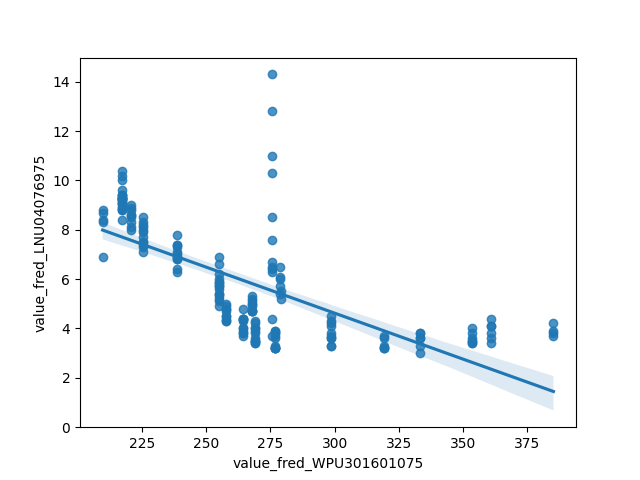
\includegraphics[scale = 0.9]{plots/plot_2024-12-12.png}
\caption{Regression Plot for 2024-12-12}
\end{figure}
\newpage

\section{Date: 2024-12-13}
\noindent \textbf{Series ID: CPACPOP} 

\noindent This series is titled Resident Population in the Pacific Census Division and has a frequency of Annual. The units are Thousands of Persons and the seasonal adjustment is Not Seasonally Adjusted.The observation start date is 1900-01-01 and the observation end date is 2023-01-01.The popularity of this series is 2. \\ 

\noindent \textbf{Series ID: A371RD3Q086SBEA} 

\noindent This series is titled Private inventories (implicit price deflator) and has a frequency of Quarterly. The units are Index 2017=100 and the seasonal adjustment is Seasonally Adjusted.The observation start date is 1947-01-01 and the observation end date is 2024-07-01.The popularity of this series is 1. \\ 

\subsection{Regression Tables and Plots}
\begin{center}
\begin{tabular}{lclc}
\toprule
\textbf{Dep. Variable:}       & value\_fred\_A371RD3Q086SBEA & \textbf{  R-squared:         } &     0.926   \\
\textbf{Model:}               &             OLS              & \textbf{  Adj. R-squared:    } &     0.925   \\
\textbf{Method:}              &        Least Squares         & \textbf{  F-statistic:       } &     943.3   \\
\textbf{Date:}                &       Fri, 13 Dec 2024       & \textbf{  Prob (F-statistic):} &  3.16e-44   \\
\textbf{Time:}                &           11:39:24           & \textbf{  Log-Likelihood:    } &   -274.41   \\
\textbf{No. Observations:}    &                77            & \textbf{  AIC:               } &     552.8   \\
\textbf{Df Residuals:}        &                75            & \textbf{  BIC:               } &     557.5   \\
\textbf{Df Model:}            &                 1            & \textbf{                     } &             \\
\textbf{Covariance Type:}     &          nonrobust           & \textbf{                     } &             \\
\bottomrule
\end{tabular}
\begin{tabular}{lcccccc}
                              & \textbf{coef} & \textbf{std err} & \textbf{t} & \textbf{P$> |$t$|$} & \textbf{[0.025} & \textbf{0.975]}  \\
\midrule
\textbf{const}                &     -26.4468  &        2.936     &    -9.007  &         0.000        &      -32.296    &      -20.597     \\
\textbf{value\_fred\_CPACPOP} &       0.0024  &     7.83e-05     &    30.713  &         0.000        &        0.002    &        0.003     \\
\bottomrule
\end{tabular}
\begin{tabular}{lclc}
\textbf{Omnibus:}       & 10.077 & \textbf{  Durbin-Watson:     } &    0.170  \\
\textbf{Prob(Omnibus):} &  0.006 & \textbf{  Jarque-Bera (JB):  } &   10.038  \\
\textbf{Skew:}          &  0.763 & \textbf{  Prob(JB):          } &  0.00661  \\
\textbf{Kurtosis:}      &  3.895 & \textbf{  Cond. No.          } & 1.12e+05  \\
\bottomrule
\end{tabular}
%\caption{OLS Regression Results}
\end{center}

Notes: \newline
 [1] Standard Errors assume that the covariance matrix of the errors is correctly specified. \newline
 [2] The condition number is large, 1.12e+05. This might indicate that there are \newline
 strong multicollinearity or other numerical problems.

\begin{figure}
\centering
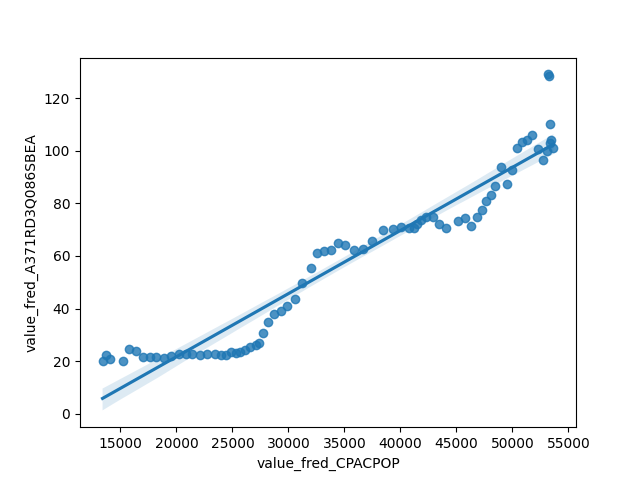
\includegraphics[scale = 0.9]{plots/plot_2024-12-13.png}
\caption{Regression Plot for 2024-12-13}
\end{figure}
\newpage

\include{tex_things/day_2024-12-14}
\section{Date: 2024-12-15}
\noindent \textbf{Series ID: COASEANZ11} 

\noindent This series is titled Import Price Index: Agriculture, forestry, fishing and hunting for Association of Southeast Asian Nations (DISCONTINUED) and has a frequency of Monthly. The units are Index 2010=100 and the seasonal adjustment is Not Seasonally Adjusted.The observation start date is 2012-06-01 and the observation end date is 2016-12-01.The popularity of this series is 1. \\ 

\noindent \textbf{Series ID: USUKFXUKM} 

\noindent This series is titled U.S. / U.K. Foreign Exchange Rate in the United Kingdom and has a frequency of Monthly. The units are U.S. Dollars to One British Pound and the seasonal adjustment is Not Seasonally Adjusted.The observation start date is 1791-01-01 and the observation end date is 2017-01-01.The popularity of this series is 23. \\ 

\subsection{Regression Tables and Plots}
\begin{center}
\begin{tabular}{lclc}
\toprule
\textbf{Dep. Variable:}          & value\_fred\_USUKFXUKM & \textbf{  R-squared:         } &     0.276   \\
\textbf{Model:}                  &          OLS           & \textbf{  Adj. R-squared:    } &     0.262   \\
\textbf{Method:}                 &     Least Squares      & \textbf{  F-statistic:       } &     20.18   \\
\textbf{Date:}                   &    Sun, 15 Dec 2024    & \textbf{  Prob (F-statistic):} &  3.85e-05   \\
\textbf{Time:}                   &        22:00:37        & \textbf{  Log-Likelihood:    } &    50.428   \\
\textbf{No. Observations:}       &             55         & \textbf{  AIC:               } &    -96.86   \\
\textbf{Df Residuals:}           &             53         & \textbf{  BIC:               } &    -92.84   \\
\textbf{Df Model:}               &              1         & \textbf{                     } &             \\
\textbf{Covariance Type:}        &       nonrobust        & \textbf{                     } &             \\
\bottomrule
\end{tabular}
\begin{tabular}{lcccccc}
                                 & \textbf{coef} & \textbf{std err} & \textbf{t} & \textbf{P$> |$t$|$} & \textbf{[0.025} & \textbf{0.975]}  \\
\midrule
\textbf{const}                   &       0.9622  &        0.128     &     7.541  &         0.000        &        0.706    &        1.218     \\
\textbf{value\_fred\_COASEANZ11} &       0.0064  &        0.001     &     4.492  &         0.000        &        0.004    &        0.009     \\
\bottomrule
\end{tabular}
\begin{tabular}{lclc}
\textbf{Omnibus:}       & 16.564 & \textbf{  Durbin-Watson:     } &    0.107  \\
\textbf{Prob(Omnibus):} &  0.000 & \textbf{  Jarque-Bera (JB):  } &   19.668  \\
\textbf{Skew:}          & -1.222 & \textbf{  Prob(JB):          } & 5.36e-05  \\
\textbf{Kurtosis:}      &  4.615 & \textbf{  Cond. No.          } &     861.  \\
\bottomrule
\end{tabular}
%\caption{OLS Regression Results}
\end{center}

Notes: \newline
 [1] Standard Errors assume that the covariance matrix of the errors is correctly specified.

\begin{figure}
\centering
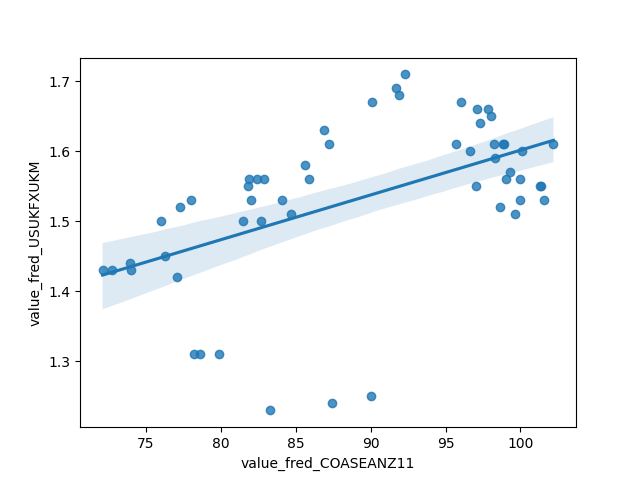
\includegraphics[scale = 0.9]{plots/plot_2024-12-15.png}
\caption{Regression Plot for 2024-12-15}
\end{figure}
\newpage

\section{Date: 2024-12-16}
\noindent \textbf{Series ID: ATNHPIUS49180Q} 

\noindent This series is titled All-Transactions House Price Index for Winston-Salem, NC (MSA) and has a frequency of Quarterly. The units are Index 1995:Q1=100 and the seasonal adjustment is Not Seasonally Adjusted.The observation start date is 1979-04-01 and the observation end date is 2024-07-01.The popularity of this series is 10. \\ 

\noindent \textbf{Series ID: ATNHPIUS16820Q} 

\noindent This series is titled All-Transactions House Price Index for Charlottesville, VA (MSA) and has a frequency of Quarterly. The units are Index 1995:Q1=100 and the seasonal adjustment is Not Seasonally Adjusted.The observation start date is 1983-07-01 and the observation end date is 2024-07-01.The popularity of this series is 11. \\ 

\subsection{Regression Tables and Plots}
\begin{center}
\begin{tabular}{lclc}
\toprule
\textbf{Dep. Variable:}              & value\_fred\_ATNHPIUS16820Q & \textbf{  R-squared:         } &     0.930   \\
\textbf{Model:}                      &             OLS             & \textbf{  Adj. R-squared:    } &     0.930   \\
\textbf{Method:}                     &        Least Squares        & \textbf{  F-statistic:       } &     2172.   \\
\textbf{Date:}                       &       Mon, 16 Dec 2024      & \textbf{  Prob (F-statistic):} &  3.81e-96   \\
\textbf{Time:}                       &           14:29:36          & \textbf{  Log-Likelihood:    } &   -745.73   \\
\textbf{No. Observations:}           &               165           & \textbf{  AIC:               } &     1495.   \\
\textbf{Df Residuals:}               &               163           & \textbf{  BIC:               } &     1502.   \\
\textbf{Df Model:}                   &                 1           & \textbf{                     } &             \\
\textbf{Covariance Type:}            &          nonrobust          & \textbf{                     } &             \\
\bottomrule
\end{tabular}
\begin{tabular}{lcccccc}
                                     & \textbf{coef} & \textbf{std err} & \textbf{t} & \textbf{P$> |$t$|$} & \textbf{[0.025} & \textbf{0.975]}  \\
\midrule
\textbf{const}                       &     -45.5379  &        5.001     &    -9.105  &         0.000        &      -55.414    &      -35.662     \\
\textbf{value\_fred\_ATNHPIUS49180Q} &       1.5958  &        0.034     &    46.610  &         0.000        &        1.528    &        1.663     \\
\bottomrule
\end{tabular}
\begin{tabular}{lclc}
\textbf{Omnibus:}       & 35.189 & \textbf{  Durbin-Watson:     } &    0.034  \\
\textbf{Prob(Omnibus):} &  0.000 & \textbf{  Jarque-Bera (JB):  } &    7.737  \\
\textbf{Skew:}          & -0.020 & \textbf{  Prob(JB):          } &   0.0209  \\
\textbf{Kurtosis:}      &  1.940 & \textbf{  Cond. No.          } &     420.  \\
\bottomrule
\end{tabular}
%\caption{OLS Regression Results}
\end{center}

Notes: \newline
 [1] Standard Errors assume that the covariance matrix of the errors is correctly specified.

\begin{figure}
\centering
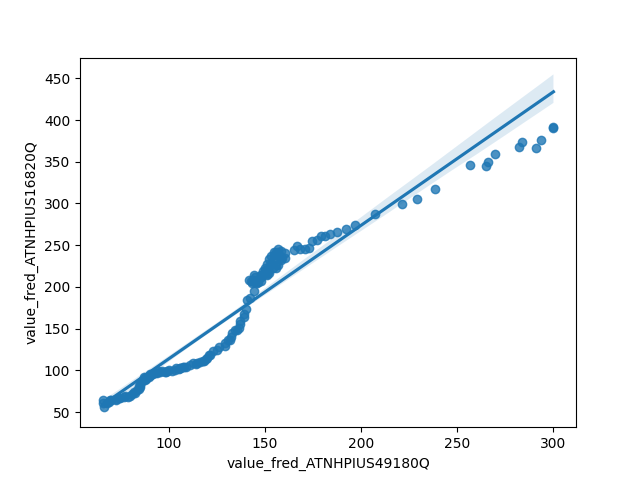
\includegraphics[scale = 0.9]{plots/plot_2024-12-16.png}
\caption{Regression Plot for 2024-12-16}
\end{figure}
\newpage

\section{Date: 2024-12-17}
\noindent \textbf{Series ID: STTMINWGAK} 

\noindent This series is titled State Minimum Wage Rate for Alaska and has a frequency of Annual. The units are Dollars per Hour and the seasonal adjustment is Not Seasonally Adjusted.The observation start date is 1968-01-01 and the observation end date is 2024-01-01.The popularity of this series is 29. \\ 

\noindent \textbf{Series ID: TLPBLCONS} 

\noindent This series is titled Total Public Construction Spending: Total Construction in the United States and has a frequency of Monthly. The units are Millions of Dollars and the seasonal adjustment is Seasonally Adjusted Annual Rate.The observation start date is 1993-01-01 and the observation end date is 2024-10-01.The popularity of this series is 36. \\ 

\subsection{Regression Tables and Plots}
\begin{center}
\begin{tabular}{lclc}
\toprule
\textbf{Dep. Variable:}          & value\_fred\_TLPBLCONS & \textbf{  R-squared:         } &     0.875   \\
\textbf{Model:}                  &          OLS           & \textbf{  Adj. R-squared:    } &     0.871   \\
\textbf{Method:}                 &     Least Squares      & \textbf{  F-statistic:       } &     210.3   \\
\textbf{Date:}                   &    Tue, 17 Dec 2024    & \textbf{  Prob (F-statistic):} &  4.28e-15   \\
\textbf{Time:}                   &        10:24:10        & \textbf{  Log-Likelihood:    } &   -376.14   \\
\textbf{No. Observations:}       &             32         & \textbf{  AIC:               } &     756.3   \\
\textbf{Df Residuals:}           &             30         & \textbf{  BIC:               } &     759.2   \\
\textbf{Df Model:}               &              1         & \textbf{                     } &             \\
\textbf{Covariance Type:}        &       nonrobust        & \textbf{                     } &             \\
\bottomrule
\end{tabular}
\begin{tabular}{lcccccc}
                                 & \textbf{coef} & \textbf{std err} & \textbf{t} & \textbf{P$> |$t$|$} & \textbf{[0.025} & \textbf{0.975]}  \\
\midrule
\textbf{const}                   &   -5.087e+04  &      2.2e+04     &    -2.313  &         0.028        &    -9.58e+04    &    -5961.472     \\
\textbf{value\_fred\_STTMINWGAK} &    4.064e+04  &     2802.081     &    14.503  &         0.000        &     3.49e+04    &     4.64e+04     \\
\bottomrule
\end{tabular}
\begin{tabular}{lclc}
\textbf{Omnibus:}       &  0.827 & \textbf{  Durbin-Watson:     } &    0.502  \\
\textbf{Prob(Omnibus):} &  0.661 & \textbf{  Jarque-Bera (JB):  } &    0.863  \\
\textbf{Skew:}          &  0.329 & \textbf{  Prob(JB):          } &    0.650  \\
\textbf{Kurtosis:}      &  2.536 & \textbf{  Cond. No.          } &     31.1  \\
\bottomrule
\end{tabular}
%\caption{OLS Regression Results}
\end{center}

Notes: \newline
 [1] Standard Errors assume that the covariance matrix of the errors is correctly specified.

\begin{figure}
\centering
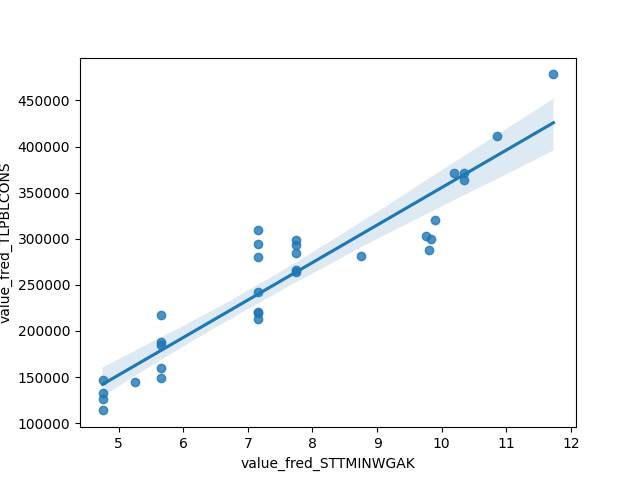
\includegraphics[scale = 0.9]{plots/plot_2024-12-17.png}
\caption{Regression Plot for 2024-12-17}
\end{figure}
\newpage

\section{Date: 2024-12-18}
\noindent \textbf{Series ID: HNOCREQ027S} 

\noindent This series is titled Households and nonprofit organizations; compensation of employees received, Flow (DISCONTINUED) and has a frequency of Quarterly. The units are Millions of Dollars and the seasonal adjustment is Seasonally Adjusted Annual Rate.The observation start date is 1946-10-01 and the observation end date is 2017-10-01.The popularity of this series is 1. \\ 

\noindent \textbf{Series ID: RINV} 

\noindent This series is titled Real Investment and has a frequency of Quarterly. The units are Billions of Chained 2012 Dollars and the seasonal adjustment is Seasonally Adjusted.The observation start date is 1947-01-01 and the observation end date is 2023-10-01.The popularity of this series is 2. \\ 

\subsection{Regression Tables and Plots}
\begin{center}
\begin{tabular}{lclc}
\toprule
\textbf{Dep. Variable:}           & value\_fred\_RINV & \textbf{  R-squared:         } &     0.983   \\
\textbf{Model:}                   &        OLS        & \textbf{  Adj. R-squared:    } &     0.983   \\
\textbf{Method:}                  &   Least Squares   & \textbf{  F-statistic:       } & 1.522e+04   \\
\textbf{Date:}                    &  Wed, 18 Dec 2024 & \textbf{  Prob (F-statistic):} & 1.87e-237   \\
\textbf{Time:}                    &      12:03:22     & \textbf{  Log-Likelihood:    } &   -1764.7   \\
\textbf{No. Observations:}        &          269      & \textbf{  AIC:               } &     3533.   \\
\textbf{Df Residuals:}            &          267      & \textbf{  BIC:               } &     3541.   \\
\textbf{Df Model:}                &            1      & \textbf{                     } &             \\
\textbf{Covariance Type:}         &     nonrobust     & \textbf{                     } &             \\
\bottomrule
\end{tabular}
\begin{tabular}{lcccccc}
                                  & \textbf{coef} & \textbf{std err} & \textbf{t} & \textbf{P$> |$t$|$} & \textbf{[0.025} & \textbf{0.975]}  \\
\midrule
\textbf{const}                    &     128.9559  &       15.231     &     8.467  &         0.000        &       98.968    &      158.944     \\
\textbf{value\_fred\_HNOCREQ027S} &       0.0004  &     3.33e-06     &   123.369  &         0.000        &        0.000    &        0.000     \\
\bottomrule
\end{tabular}
\begin{tabular}{lclc}
\textbf{Omnibus:}       & 10.569 & \textbf{  Durbin-Watson:     } &    0.032  \\
\textbf{Prob(Omnibus):} &  0.005 & \textbf{  Jarque-Bera (JB):  } &   14.122  \\
\textbf{Skew:}          & -0.303 & \textbf{  Prob(JB):          } & 0.000858  \\
\textbf{Kurtosis:}      &  3.945 & \textbf{  Cond. No.          } & 6.67e+06  \\
\bottomrule
\end{tabular}
%\caption{OLS Regression Results}
\end{center}

Notes: \newline
 [1] Standard Errors assume that the covariance matrix of the errors is correctly specified. \newline
 [2] The condition number is large, 6.67e+06. This might indicate that there are \newline
 strong multicollinearity or other numerical problems.

\begin{figure}
\centering
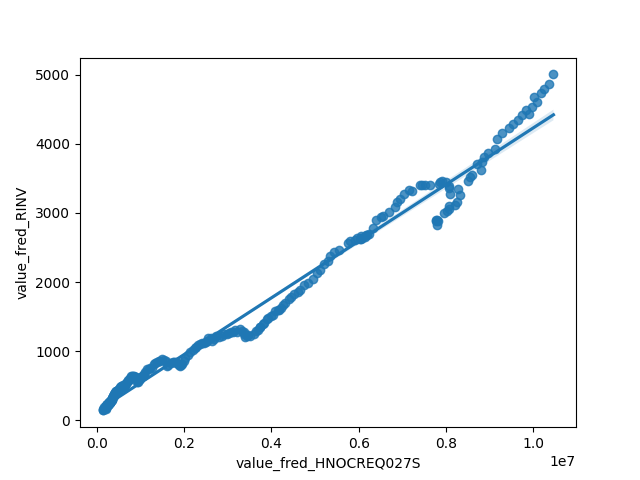
\includegraphics[scale = 0.9]{plots/plot_2024-12-18.png}
\caption{Regression Plot for 2024-12-18}
\end{figure}
\newpage


\end{document}
